\documentclass[a4paper]{article}
\usepackage[utf8]{inputenc}
\usepackage[spanish]{babel}
% \usepackage{hyperref}
\usepackage{graphicx}


\title{Interacción Persona-Computadora}
\author{Sergio Alonso Pascual \\ Adrián Arroyo Calle \\ Irene Caldelas Fernández \\ Cristina de la Torre Cáceres}
\date{Mayo 2018}


\begin{document}

\maketitle

\tableofcontents

\pagebreak

\section{Introducción}

En el mundo actual, los usuarios quieren poder escuchar sus programas de radio en cualquier momento, previamente grabados. Con este nuevo medio de comunicación conocido como \textit{podcast}, han surgido diferentes aplicaciones que buscan ser amigables con el usuario y que actúen de forma lo más transparente posible, rompiendo la barrera entre creadores de contenido y consumidores. De ahí surge, Sintonízame, una aplicación multidispositivo que permite a los usuarios escuchar sus podcasts preferidos de sus locutores preferidos cuando quieran y donde quieran, con la máxima calidad posible.

\begin{center}
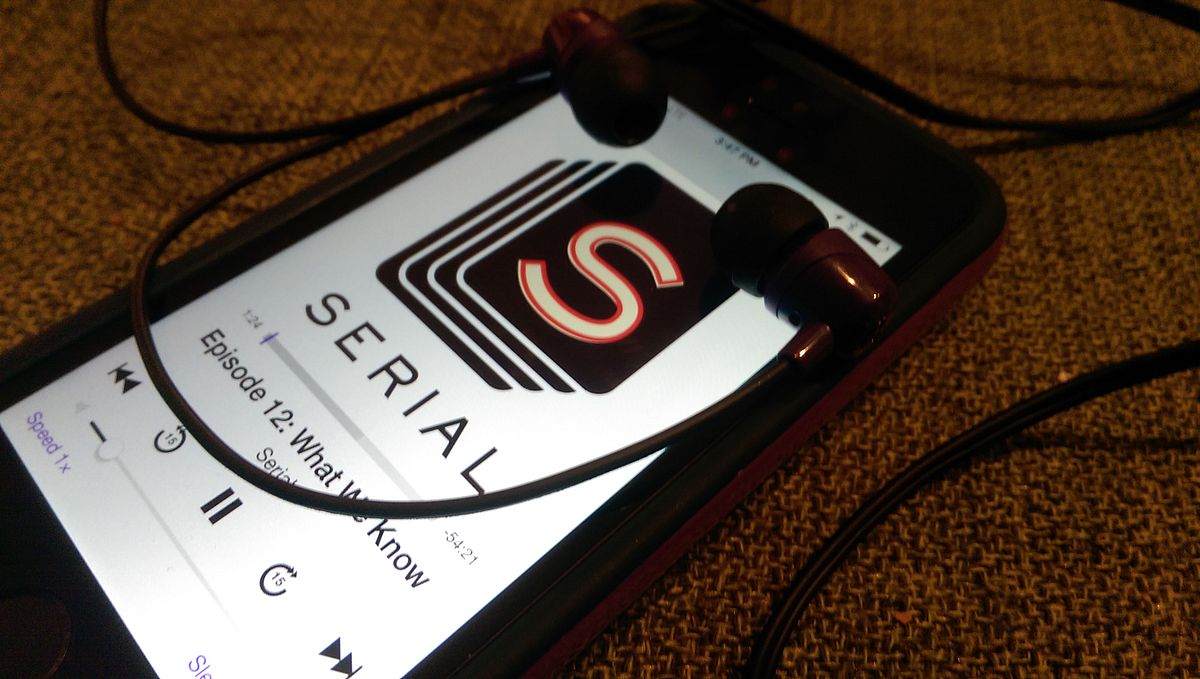
\includegraphics[width=0.7\columnwidth]{Podcast.jpg}
\end{center}

\section{Requisitos funcionales de la aplicación}

La aplicación diseñada, permite escuchar podcasts, suscribirse a canales creadores de podcasts para recibir novedades, crear playlists de podcasts y mostrar sugerencias de nuevos podcasts.

\section{Prototipado de bajo coste}

Para realizar las primeras pruebas de usabilidad, se ha diseñado un prototipo con materiales reciclados y de bajo coste.

Para el prototipo de Sintonízame hemos hecho un teléfono falso, al que le vamos cambiando las pantallas con cartulinas. El teléfono falso está hecho con una caja de cartón (que en tiempos pasados era de chocolate) al que se le ha recortado una ventana de tamaño amplio, para simular las pantallas táctiles de los \textit{smartphones} actuales. Aunque más voluminoso que un teléfono real, la experiencia en la mano es similar y el peso es parecido. Las pantallas, cuyas dimensiones exactas son de 9x16,5 centímetros, se ajustan a la ventana de la maqueta, de 9x15,5. Se deja un centímetro para poder cambiar entre pantallas con mayor facilidad. Las cartulinas aportan consistencia extra ya que no se doblan con tanta facilidad.

Además, la caja dispone de una ranura para introducir los diferentes teclados que la aplicación puede pedir para que el usuario introduzca datos. Estos teclados, solo aparecen al encontrarse un campo de texto, para no malgastar espacio de la pantalla innecesariamente.

Para el prototipo hemos diseñado un logo con lettering, salvo eso, que es por motivos estéticos, el resto de la aplicación usa tipografías claras para que los usuarios no deban esforzarse mucho en leer los botones y opciones.

La interfaz consta de una barra inferior que permite acceder rápidamente a las acciones más comunes, la barra no tiene más de 3 opciones (Mi Perfil, Buscar y Suscripciones) ya que buscamos sencillez. La ley de Fitts además nos indica que el lugar adecuado para un menú de este tipo es justamente en un borde de la pantalla. El resto de la pantalla es la acción principal que se esté realizando: escuchar un podcast, revisar las sugerencias, encontrar las novedades,...

En estas pantallas se prima el contenido visual y unos pocos botones de acción, grandes, muy en línea con otras aplicaciones similares de reproducción de contenido multimedia: reproducir/pausa, ajustes de sonido (volumen, calidad, etc). En la pantalla de novedades existe una barra superior de búsqueda, esta incluye a su vez un botón para activar filtros de búsqueda, referentes a género, idioma, fecha, ...

Inicialmente diseñamos los bocetos pensando en una interfaz en horizontal, acorde al resto de dispositivos con los que es compatible la aplicación, posteriormente decidimos que en un teléfono era mucho más conveniente soportar el modo vertical en primer (y de momento único) lugar. Esto es debido a que la mayoría de aplicaciones trabajan en ese modo y el launcher desde el que se lanza la aplicación también suele ser vertical. Bocetos en \ref{bocetos}


\section{Resultados}

\section{Conclusiones}

\section{Bibliografía}

\appendix

\section{Apéndices}

\subsection{Bocetos}
\label{bocetos}

\begin{center}
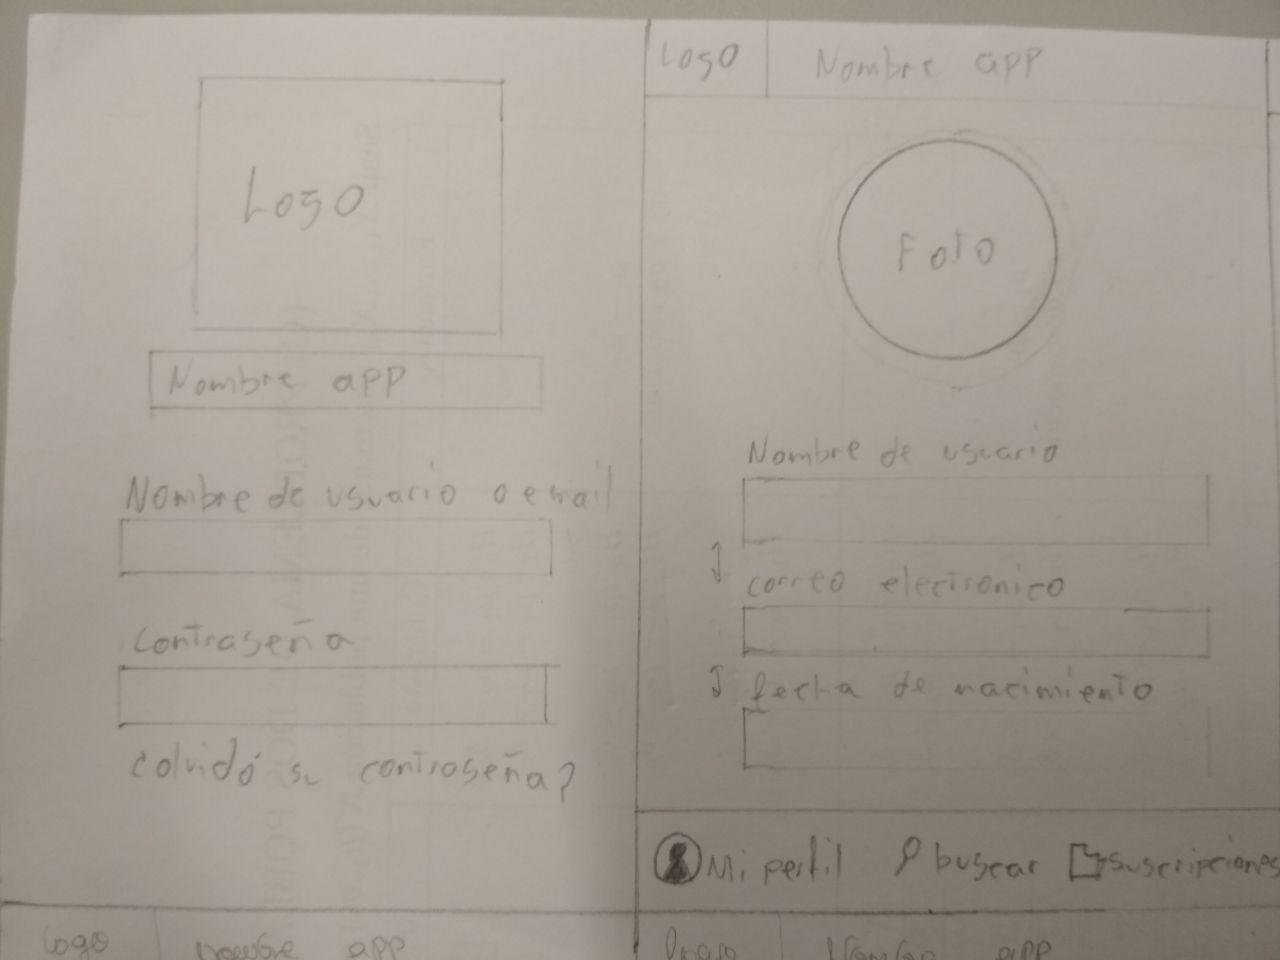
\includegraphics[width=0.7\columnwidth]{Boceto-1.jpg} \\
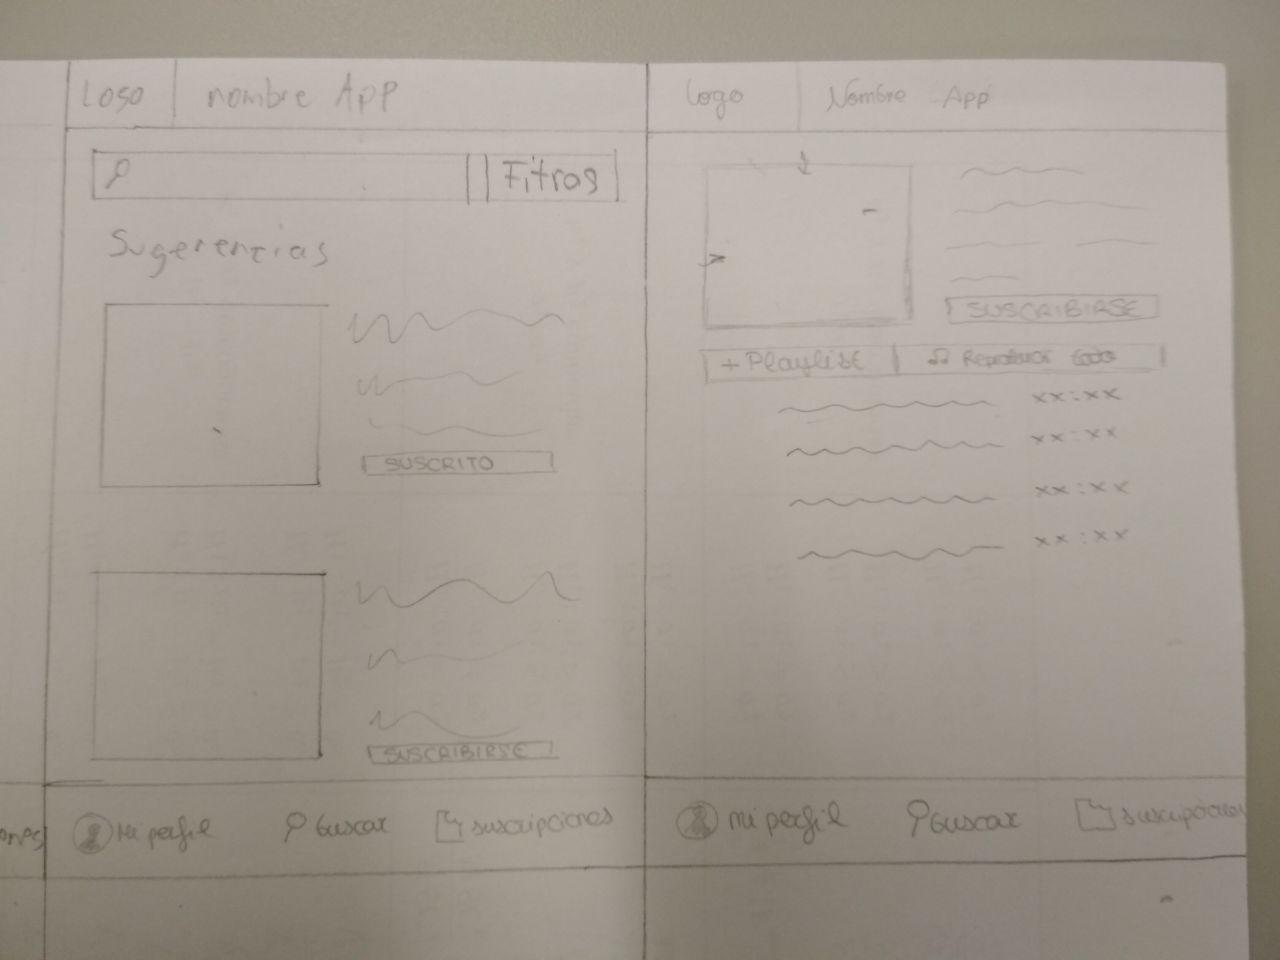
\includegraphics[width=0.7\columnwidth]{Boceto-2.jpg} \\
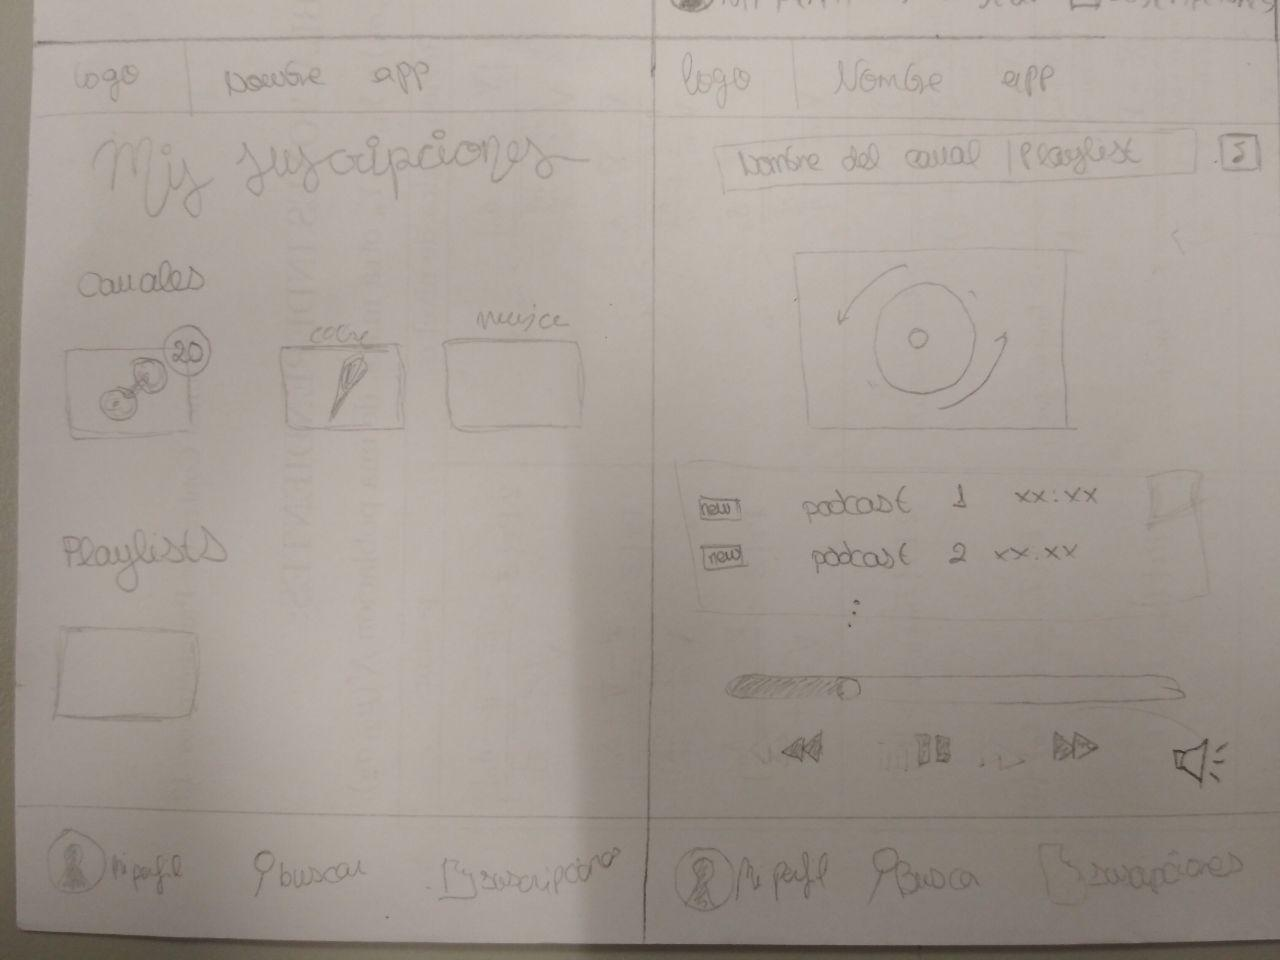
\includegraphics[width=0.7\columnwidth]{Boceto-3.jpg} \\
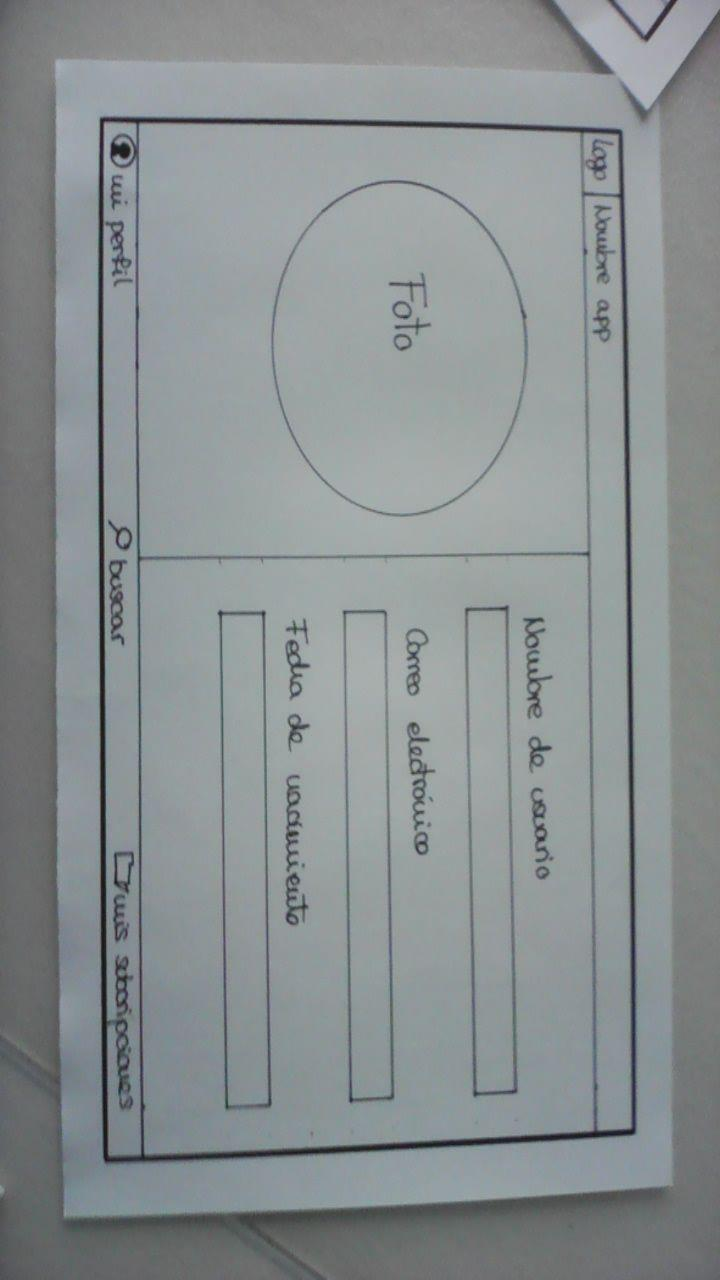
\includegraphics[width=0.7\columnwidth]{Boceto-4.jpg} \\
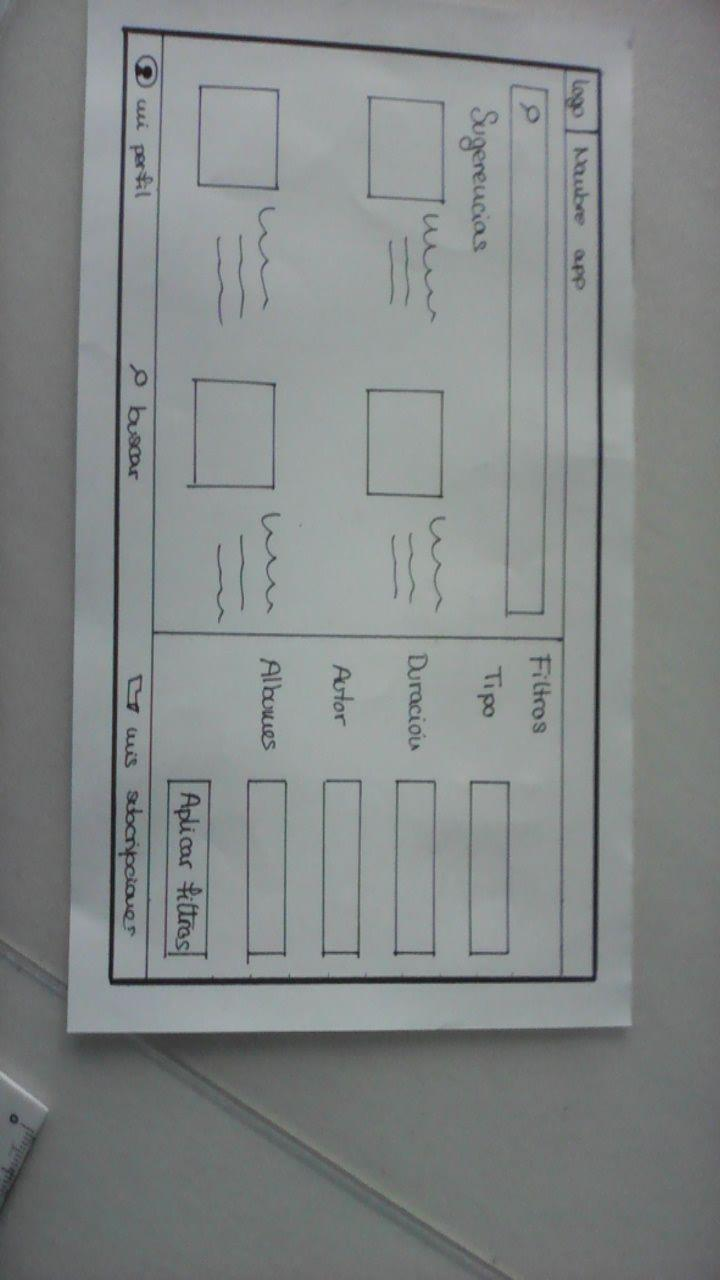
\includegraphics[width=0.7\columnwidth]{Boceto-5.jpg} \\
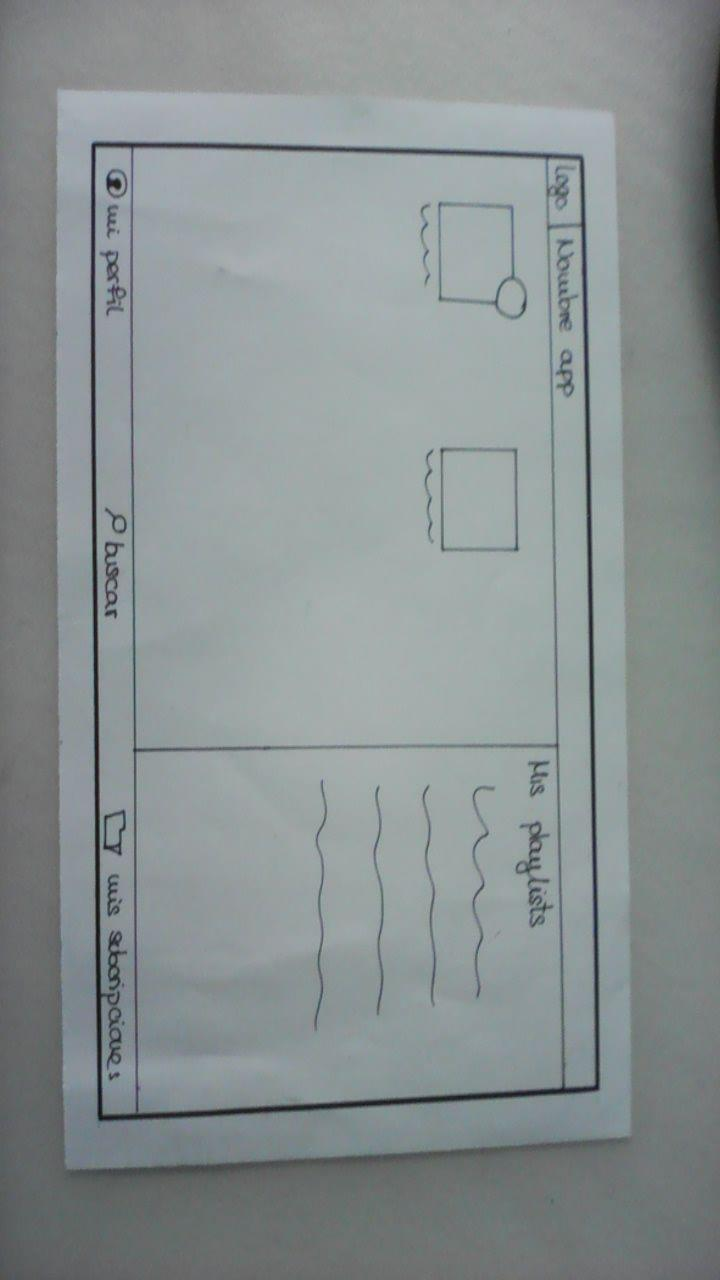
\includegraphics[width=0.7\columnwidth]{Boceto-6.jpg}
\end{center}



\end{document}
